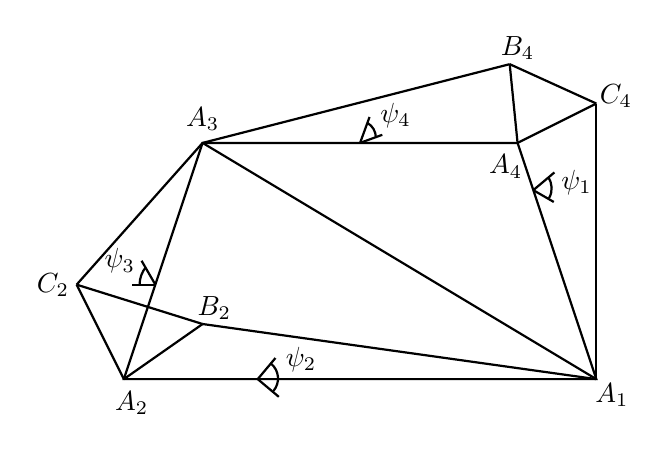
\begin{tikzpicture}[>=latex]              %\draw[help lines] (0,0) grid (15,10);

        \coordinate (a1) at (9, 4);
        \coordinate (a2) at (3, 4);
        \coordinate (a3) at (4, 7);
        \coordinate (a4) at (8, 7);
        \coordinate (b1) at (10, 4.5);
        \coordinate (c1) at (9.5, 3);
        \coordinate (b2) at (4, 4.7);
        \coordinate (c2) at (2.4, 5.2);
        \coordinate (b3) at (3.2, 7.7);
        \coordinate (c3) at (4.1, 8);
        \coordinate (b4) at (7.9, 8);
        \coordinate (c4) at (9, 7.5);

        \draw[thick] (a1) -- (a2) -- (a3) -- (a4) -- cycle;
        
        \draw[thick] (a3) -- (a1);
        \draw[thick] (a2) -- (b2);
        \draw[thick] (a2) -- (c2);
        \draw[thick] (a4) -- (b4);
        \draw[thick] (a4) -- (c4);
        \draw[thick] (a1) -- (c4); 
        \draw[thick] (a1) -- (b2);
        \draw[thick] (c2) -- (a3);
        \draw[thick] (b4) -- (a3);
        \draw[thick] (b2) -- (c2);
        \draw[thick] (b4) -- (c4);

        \draw (a1) + (0.2, -0.2) node {$A_1$};
        
        \draw (a2) + (0.1, -0.3) node {$A_2$};
        \draw (b2) + (0.15, 0.2) node {$B_2$};
        \draw (c2) + (-0.3, 0) node {$C_2$};
        
        \draw (a3) + (0, 0.3) node {$A_3$};
        
        \draw (a4) + (-0.15, -0.3) node {$A_4$};
        \draw (b4) + (0.1, 0.2) node {$B_4$};
        \draw (c4) + (.25, .1) node {$C_4$};

        \coordinate (psi2) at (4.7, 4);
        \draw[thick, , rotate around = {-40:(psi2)}] (psi2) -- + (0, 0.35);
        \draw[thick, rotate around = {-40:(psi2)}] (psi2) -- + (0.35, 0);
        \draw[thick] (psi2) + (0.2, -0.15) arc (-40:50:7pt);
        \draw (psi2) + (0.55, 0.25) node {$\psi_2$};

        \coordinate (psi3) at (3.4, 5.2);
        %\draw (psi3) node {\textbullet};
        \draw[thick, , rotate around = {30:(psi3)}] (psi3) -- + (0, 0.35);
        \draw[thick, , rotate around = {0:(psi3)}] (psi3) -- + (-0.3, 0);
        \draw[thick] (psi3) + (-0.2, 0) arc (180:141:10pt);
        \draw (psi3) + (-0.45, 0.3) node {$\psi_3$};

        \coordinate (psi1) at (8.2, 6.4);
        %\draw (psi4) node {\textbullet};
        \draw[thick, rotate around = {-50:(psi1)}] (psi1) -- + (0, 0.35);
        \draw[thick, rotate around = {-30:(psi1)}] (psi1) -- + (0.3, 0);
        \draw[thick] (psi1) + (0.2, -0.1) arc (-30:36:7pt);
        \draw (psi1) + (.55, .1) node {$\psi_1$};

        \coordinate (psi4) at (6, 7);
        %\draw (psi4) node {\textbullet};
        \draw[thick, rotate around = {-20:(psi4)}] (psi4) -- + (0, 0.35);
        \draw[thick, rotate around = {20:(psi4)}] (psi4) -- + (0.3, 0);
        \draw[thick] (psi4) + (0.2, .07) arc (0:60:6pt);
        \draw (psi4) + (.45, .35) node {$\psi_4$};
        
    \end{tikzpicture}